\documentclass[11pt,a5paper]{article}
\usepackage[utf8]{inputenc}
\usepackage[english]{babel}
\usepackage{amsmath}
\usepackage{amsthm}
\usepackage{amsfonts}
\usepackage[margin=0.47in]{geometry}
\usepackage{graphicx}

\newtheorem{theorem}{Example}
\newtheorem{exercise}{Exercise}
\newtheorem*{Theorem}{Theorem}

\title{\textbf{Fractals and the Chaos Game}}
\date{Week 3}
\author{Jonas Wolter}

\begin{document}
\maketitle

\noindent We have seen two different possibilities to generate fractals yet. One uses more-or-less descriptions on how a fractal is produced. The other one uses L-systems. \\ 
Interstingly, there is a third method to generate fractals using a probalistic algorithm which is known as the \emph{Chaos Game}.
As an example, the following algorithm produces the Sierpinski Triangle which we have already seen when we were looking at L-systems.

\begin{enumerate}

\item {Draw an equilateral triangle, labelling the vertices \emph{A},\emph{ B}, and \emph{C}.}
\item {Draw a point anywhere inside the triangle.}
\item {Choose one of \emph{A},\emph{ B} or \emph{C} with equal probability (for example by rolling a standard die and
choosing \emph{A} on a roll of 1 or 2, \emph{B} on 3 or 4 and \emph{C} on 5 or 6).}
\item {Move half way from your point towards the chosen vertex and draw another point.}
\item {Repeatedly apply steps 3 and 4, each time starting from the point just drawn.}

\end{enumerate}

\begin{figure}[h!]
\begin{center}
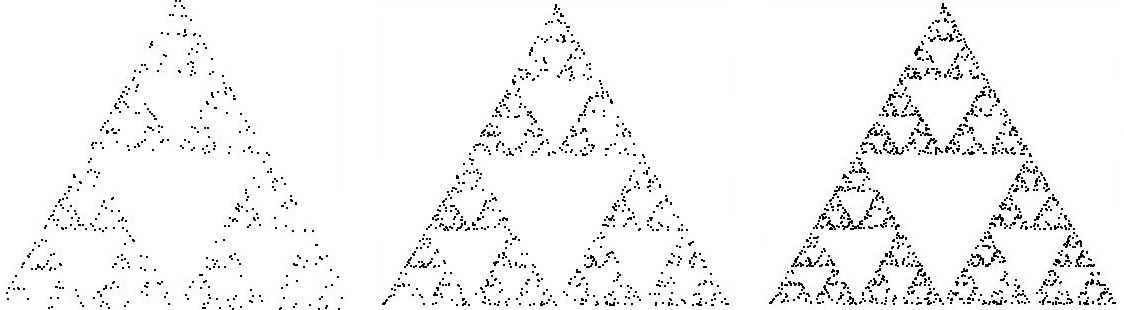
\includegraphics[width=9cm]{sierpinski-3panel.jpg}
\caption{Chaos Game after 500, 1000 and 2000 iterations.}
\end{center}
\end{figure}

\begin{exercise}
Why does the given algorithm costruct the Sierpinski triangle?
\end{exercise}

\begin{exercise}
Is the randomness of every step necessary for the construction of the Sierpinksi triangle? In other words: Can we generate a sequence of choice of vertices that also generates the Sierpinksi triangle?
\end{exercise}

\begin{exercise}
What happens if we start with an initial point outside the triangle? What happens if not all vertices are chosen with the same probability?
\end{exercise}

\noindent Seeing this quite interesting result of the Chaos game in a triangle gives rise to the question what happens in other n-gons. Unfortunately the result is not always nice and sometimes the needed values are really awful, but one pretty fasciting figure may be obtained in the following exercise.\\

\begin{exercise}
Try to figure out the result of the Chaos game in an hexagon when one moves in every step $\frac{1}{3}$ of the current distance to the chosen vertex?
\end{exercise}

\end {document}